\section{Bancos de Dados}

\subsection{Transações}
Falar em bancos de dados distribuídos implica falar em bancos transacionais e P2P.

\begin{frame}{Operações Atômicas}
Falar em bancos de dados distribuídos implica falar em bancos Relacionais/Transactionais e P2P.

Falar em bancos transacionais, implica falar ACID!
\end{frame}


\begin{frame}{Operações Atômicas}
No modelo de Máquinas de Estados Replicadas, operações são enviadas para as réplicas, que as executam em ordem, deterministicamente e também \emph{atomicamente}. Isto é, cada operação é ou executada independentemente das outras e por completo, ou não é executada.
\end{frame}

\begin{frame}{Conjuntos de Operações}
Mesmo com Operações Atômicas, frequentemente queremos/precisamos agrupar operações tal que
\begin{itemize}
	\item \alert{todas ou nenhuma} sejam executadas
	\item mesmo na presença de falhas.
\end{itemize}

\pause \emph{Atomicidade}.
\end{frame}




\begin{frame}{Memória Estável}
Para que os efeitos de operações não sejam esquecidos, eles precisam ser armazenados em \emph{memória estável} como
\begin{itemize}
	\item HD -- Hard Drives
	\item SSD -- Solid State Drives
	\item NVRAM -- Non Volatile Ram
\end{itemize} 

\pause \emph{Durabilidade}.
\end{frame}



\begin{frame}{Transações}
\begin{itemize}
	\item \alert{Atomicidade} -- Todas as operações ou nenhuma.
	\item Consistência -- Os dados transitam de estado válido para estado válido.
	\item Isolamento -- Transações não interferem umas nas outras.
	\item \alert{Durabilidade} -- Efeitos não são esquecidos.
\end{itemize}
\end{frame}

\begin{frame}{O Banco}
Conta C
\begin{itemize}
	\item C.\alert{get}Saldo()
	\item C.\alert{set}Saldo(montante)
\end{itemize}
\end{frame}

\begin{frame}[fragile]{Transação}
Mova 10\% do saldo de X, de Y para X.
\begin{verbatim}
T1: a -> b
sB = b.getSaldo()
     b.setSaldo(sB*1.1)
sA = a.getSaldo()                          
     a.setSaldo(sA-sB*0.1)
\end{verbatim}
\end{frame}

\begin{frame}[fragile]{Transação}
Qual o saldo total das contas?
\begin{verbatim}
T2: a + b
sA = a.getSaldo()
sB = b.getSaldo()
sT = sA + sB
\end{verbatim}
\end{frame}


\begin{frame}[fragile]{Execução Concorrente}
Execução concorrente de T1 e T2?
\begin{verbatim}
T1                           T2
sB = b.getSaldo()
                             sA = a.getSaldo()
     b.setSaldo(sB*1.1)
                             sB = b.getSaldo()
sA = a.getSaldo()                          
     a.setSaldo(sA-sB*0.1)
                             sT = sA+sB
\end{verbatim}

\pause Dados não finais ``vazaram''. \emph{Dirty Read}. 

\pause Falta \emph{Isolamento}.
\end{frame}

Pode levar a mais que um resultado errado. Pode deixar o BD em estado inválido.

\begin{frame}[fragile]{Execução Concorrente}
Mova 10\% do saldo de X, de Y para X.
\begin{verbatim}
T1                       T1
sB = b.getSaldo()
                          sB = b.getSaldo()
                               b.setSaldo(sB*1.1)
     b.setSaldo(sB*1.1)                                        
                          sA = a.getSaldo()                          
                               a.setSaldo(sA-sB*0.1)
sA = a.getSaldo()                          
     a.setSaldo(sA-sB*0.1)
\end{verbatim}

\pause \verb|sB*0.1| foi perdido. \emph{Lost Update}

\pause Perdeu \emph{Consistência}
\end{frame}



\begin{frame}{Solução?!}
Para garantir Isolamento
\begin{itemize}
	\item Execuções dos conjuntos não podem se sobrepor.
	\item Execute um conjunto de operações por vez, serialmente!
	\item Garantirá também Consistência
\end{itemize}


\pause \alert{Que tal?}
\pause Limite a concorrência de transações.
\end{frame}

\subsection{Equivalência Serial}

\begin{frame}{Concorrência}
Além de ACID, queremos o máximo de \emph{concorrência} para garantir o melhor \emph{desempenho}.\pause

Queremos uma execução das transações semelhante à serial, mas com o desempenho de concorrente.\pause

Não queremos uma execução serial, mas uma \alert{Equivalência Serial}, isto é, que os efeitos das transações, executadas concorrentemente, sejam equivalentes aos de alguma execução serial destas transações.
\end{frame}

\begin{frame}{Equivalência Serial}
Preocupe-se com Operações Conflitantes
\begin{itemize}
	\item Transações diferentes
	\item Uma é escrita
	\item Mesmo dado
\end{itemize}

Duas execuções (de transações) são equivalentes se
\begin{itemize}
	\item as transações tem as mesmas operações
	\item quaisquer duas operações conflitantes são executadas na mesma ordem nas duas execuções
\end{itemize}

Uma execução tem Equivalência Serial se é equivalente a alguma execução serial das transações.
\end{frame}

\begin{frame}{Equivalência Serial}
Escalone operações concorrentemente, de forma a obter o melhor desempenho, mas de forma a manter Equivalência Serial.
\end{frame}

Esta definição difícil de ser testada. Algo mais simples?

\begin{frame}{Equivalência Serial}
\begin{itemize}
	\item Como demonstrar Equivalência Serial? 
	\item Tenho que testar todas as execuções seriais e ver se uma casa com o que planejo fazer?
	\item É caro fazer este planejamento. É mais eficiente garantir por construção.
\end{itemize}
\end{frame}

\begin{frame}{Equivalência Serial}
Simplificação: A execução de duas transações tem Equivalência Serial se todos os pares de operações conflitantes entre as transações são executados na mesma ordem.
\end{frame}


\begin{frame}[fragile]{Lost Update}
Mova 10\% do saldo de X, de Y para X.
\begin{verbatim}
a -> b                     c -> b
s = b.getSaldo() [1]
                           [2]s = b.getSaldo()
                           [3]    b.setSaldo(s*1.1)
    b.setSaldo(s*1.1)[4]                                        
                                  c.setSaldo(s*0.1)
    a.setSaldo(s*0.1)
\end{verbatim}

Conflitos: 1x3:$\rightarrow$, 2x4:$\leftarrow$, 3x4:$\leftarrow$

\pause Consistência -- \verb|s*0.1| foi perdido
\end{frame}

\begin{frame}[fragile]{Lost Update}
Mova 10\% do saldo de X, de Y para X.
\begin{verbatim}
a -> b                    c -> b
                          [2] s = b.getSaldo()
                             [3]  b.setSaldo(s*1.1)
s = b.getSaldo() [1]
    b.setSaldo(s*1.1)[4]                                        
                              c.setSaldo(s*0.1)
    a.setSaldo(saldo*0.1)
\end{verbatim}

Conflitos: 1x3:$\leftarrow$, 2x4:$\leftarrow$, 3x4:$\leftarrow$
\end{frame}


\begin{frame}[fragile]{Dirty Read}
Saldo total?
\begin{verbatim}
a -> b                  a -> b
s = b.getSaldo()
    b.setSaldo(s*1.1)
    b.setSaldo(s*1.1)                                        
    a.saque(s*0.1)
                        s = b.getSaldo()
                            b.setSaldo(s*1.1)
                            b.setSaldo(s*1.1)                                        
                            a.saque(s*0.1)
\end{verbatim}
\pause Tem Equivalência Serial.

\pause Exceto se
\begin{verbatim}
abortTransaction()
\end{verbatim}
\pause Nenhuma transação que fez uma dirty read pode comitar. Logo, aborte a transação da direita.
\end{frame}


\begin{frame}{Aborto em Cascata}
T1 faz uma escrita. T2 lê o que T1 escreveu e faz outra escrita. T3 lê o que T2 escreveu e faz outra escrita. T4 lê o que... \alert{T1 aborta.}
\end{frame}

\begin{frame}{Dirty Read}
Como lidar?
\begin{itemize}
	\item Suspenda a transação quando esta fizer dirty read.
	\item Se transação foi abortada, todas as suspensas (que leram dela) devem ser abortadas.
	\item Repita passo anterior.
\end{itemize}

\pause E se evitarmos dirty reads em vez de tratarmos?
\pause
\begin{itemize}
	\item Suspenda antes de fazer dirty read.
	\item Quando transação for terminada, continue execução.
\end{itemize}
\pause Abordagem leva a menor concorrência.
\end{frame}

Para nos permitir identificar transações, vamos usar o seguinte framework para operá-las.
\begin{frame}{Transações}
\begin{itemize}
	\item beginTransaction()
	\item operações
	\item commitTransaction(): Ok/NOk
	\item abortTransaction()
\end{itemize}
\end{frame}



\begin{frame}[fragile]{Escrita Prematura}
\begin{verbatim}
Saldo inicial: 100

a.setSaldo(105)
                   a.setSaldo(110)  
                   commitTransaction()
abortTransaction()
\end{verbatim}

A transação da direita não le, apenas escreve. O resultado?  O saldo volta para 100.
\end{frame}


\begin{frame}{Strict Execution}
\begin{itemize}
	\item Leituras e Escritas devem ser atrasadas até que todas as transações anteriores que contenham escritas sejam commitadas ou abortadas.
	\item Execução estrita garante Isolamento.
	\item Como implementar eficientemente?
\end{itemize}
\end{frame}


\subsection{Controle de Concorrência}

\begin{frame}{Como}
\begin{itemize}
	\item locks (pessimista): simples, mas problemático
	\item multi-versão (otimista): custo se há muitos conflitos
	\item timestamp: \alert{time} é algo complicado
\end{itemize}
\end{frame}

\subsubsection{Locks}
\begin{frame}{Locks}
Tranque todos os objetos para que outras transações não consigam ler ou escrevê-los. Destranque quando não mais necessários.

Sofre de dirty reads e escritas prematuras.

\begin{block}{Strict Two Phase Locking}
\begin{itemize}
	\item tranque quando necessário
	\item destranque ao final da transação
	\item termine a transação
\end{itemize}

\end{block}

Como aumentar a concorrência?
\end{frame}

\begin{frame}{Read-Write Locks}
\begin{itemize}
	\item dois níveis de acesso
	\item múltiplos leitores
	\item único escritor
	\item reads por ser transformados em locks
	\item writes \alert{não} podem se transformados em reads (violaria Strict Two-Phase Locking)
\end{itemize}
\end{frame}

\begin{frame}{Variantes}
\begin{itemize}
	\item Two-version locking (read/write/commit)
%	Similar idea but now with: read, write and commit locks.
%	\begin{itemize}
%		\item A read lock is allowed unless a commit lock is taken.
%		\item One write lock is allowed if no commit lock is taken (i.e. even if read locks are taken)
%		\item Written values are held local to the transaction and are not visible before commit.
%		\item A write lock can be promoted to a commit lock if there are no read locks.
%		\item When a transaction commits it tries to promote write locks to commit locks.
%	\end{itemize}
	\item Lock hierárquico (granularidades variadas)
%	locks of mixed granularity.
%	\begin{itemize}
%		\item Small locks increase concurrency
%		\item Large locks decrease overhead
%	\end{itemize}
\end{itemize}
\end{frame}

\begin{frame}{Lock -- Por quê evitar?}
\begin{itemize}
	\item Pessimista
	\item Overhead mesmo se não há conflitos
	\item Ou restritivo ou risco de deadlock
	\item Lock liberado somente no final, para evitar dirty reads/escrita prematura.
\end{itemize}
\end{frame}

\subsubsection{Otimista}
\begin{frame}{Abordagem mais otimista?}
\begin{itemize}
	\item Modifique uma cópia privada dos dados
	\item Na hora de terminar a transação, verifique se nenhuma transação modificou o dado, isto é,
	\item se a cópia privada ainda é válida.
	\item Substitua a cópia pública pela privada
\end{itemize}

Esta técnica é conhecida como \emph{deferred update}, pois o Update dos dados só ocorre no final, se a Validação passar.
\end{frame}

\begin{frame}{Abordagem Otimista}
\begin{itemize}
	\item Baixo overhead, se não houver conflitos
	\item Validação é rápida
	\item Update é simples
\end{itemize}

Se houver muitos conflitos, o trabalho da transação é todo desperdiçado.
\end{frame}

\begin{frame}{Validação}
Read e Write sets de quaisquer transações concorrentes deve ser disjuntos.
\begin{itemize}
	\item T1 não deve ler dados escritos por T2
	\item T2 não deve ler dados escritos por T1
	\item T1/T2 não deve escrever dados escritos por T2/T1
\end{itemize}
\includegraphics[width=.7\textwidth]{images/trans_validation}
\end{frame}

\begin{frame}{Backward Validation}
\begin{itemize}
	\item T1: transação sendo validada
	\item T2: transação já comitada.
	\item T1 não deve ler dados escritos por T2
\end{itemize}
Em caso de não validação, aborte T1

\includegraphics[width=.7\textwidth]{images/trans_validation}
\end{frame}

\begin{frame}{Forward Validation}
\begin{itemize}
	\item T1: transação sendo validada
	\item T2: transação ainda em execução
	\item T2 não deve ler dados escritos por T1
\end{itemize}
Em caso de não validação, aborte T1

\includegraphics[width=.7\textwidth]{images/trans_validation}

\pause, possivelmente nunca terminando uma transação.\\
Ou aborte T2.
\end{frame}

\subsubsection{Timestamp}
\begin{frame}{Timestamping}
\begin{itemize}
	\item Transação recebe um \emph{timestamp} no início
	\item Operações são validadas na execução
	\begin{itemize}
		\item leia somente se nenhuma transação com maior timestamp tiver escrito e comitado
		\item escreva somente se nenhuma transação com maior timestamp tiver lido e comitado
	\end{itemize}
	\item Transações ``executam na ordem do timestamp''
\end{itemize}

Como implementar?
\end{frame}

\begin{frame}{Como implementar}
\begin{itemize}
	\item Objetos tem valores \emph{tentativos}, não comitados
	\item Objetos tem versões em que foram escritos
	\item em que foram comitados
	\item e em que foram lidos
	
	\includegraphics[width=.9\textwidth]{images/timestamp1}

	\item Consistência é testado na execução da operação
	
\end{itemize}
\end{frame}

\begin{frame}{Como implementar -- Escrita}
\begin{itemize}
	\item Escritas tem sucesso somente se versão sendo escrita é maior que versões lidas
	\item Se versão sendo escrita é menor que versão já escrita, ignore e continue

	\includegraphics[width=.9\textwidth]{images/timestamp1}
\end{itemize}
\end{frame}

\begin{frame}{Como implementar -- Leitura}
\begin{itemize}
	\item Leitura com versão v tem sucesso se maior versão é comitada e menor que v ou alguma não comitada
	\item Leitura com versão v é suspensa se maior versão é não comitada e menor que v
	\includegraphics[width=.9\textwidth]{images/timestamp2}
\end{itemize}
\end{frame}

\begin{frame}{Como implementar}
\begin{itemize}
	\item Leitura com versão v é abortada se maior versão comitada é maior que v
	\includegraphics[width=.9\textwidth]{images/timestamp3}	
\end{itemize}
\end{frame}


\begin{frame}{Referências}
Inspirado nas notas de aula de Johan Montelius e Vladimir Vlassov, da disciplina ID2201 Distributed Systems, KTH Royal Institute of Technology. Imagens copiadas descaradamente de seus slides.

Também aqui, \url{https://www.cs.ucy.ac.cy/~dzeina/courses/epl446/lectures/16.pdf}
\end{frame}




\section{Bancos de Dados Distribuídos}

\subsection{Transações Distribuídas}
\begin{frame}{Bancos de Dados Transacionais Distribuídos}
Agora que relembramos como transações funcionam e temos uma noção de como podem ser implementadas em um sistema centralizado, vamos tentar entender como fazê-lo em um sistema distribuído.

\begin{itemize}
	\item Múltiplos servidores
	\item Transações em cada servidor
	\item Transações distribuídas
	\item Como obter Equivalência Serial em transações distribuídas
\end{itemize}
\end{frame}

\begin{frame}{Transação Distribuída}
\begin{itemize}
	\item beginTransaction(): tid (transaction id)
	\item operation(tid,op)
	\item endTransaction(tid): Ok/NOk
	\item abortTransaction(tid)
\end{itemize}
\end{frame}

\begin{frame}{Transações Distribuídas}
\begin{itemize}
	\item Cliente
	\item Servidor: \emph{resource managers}
	\item Servidor: \emph{transaction monitor/manager}
\end{itemize}

\begin{center}
	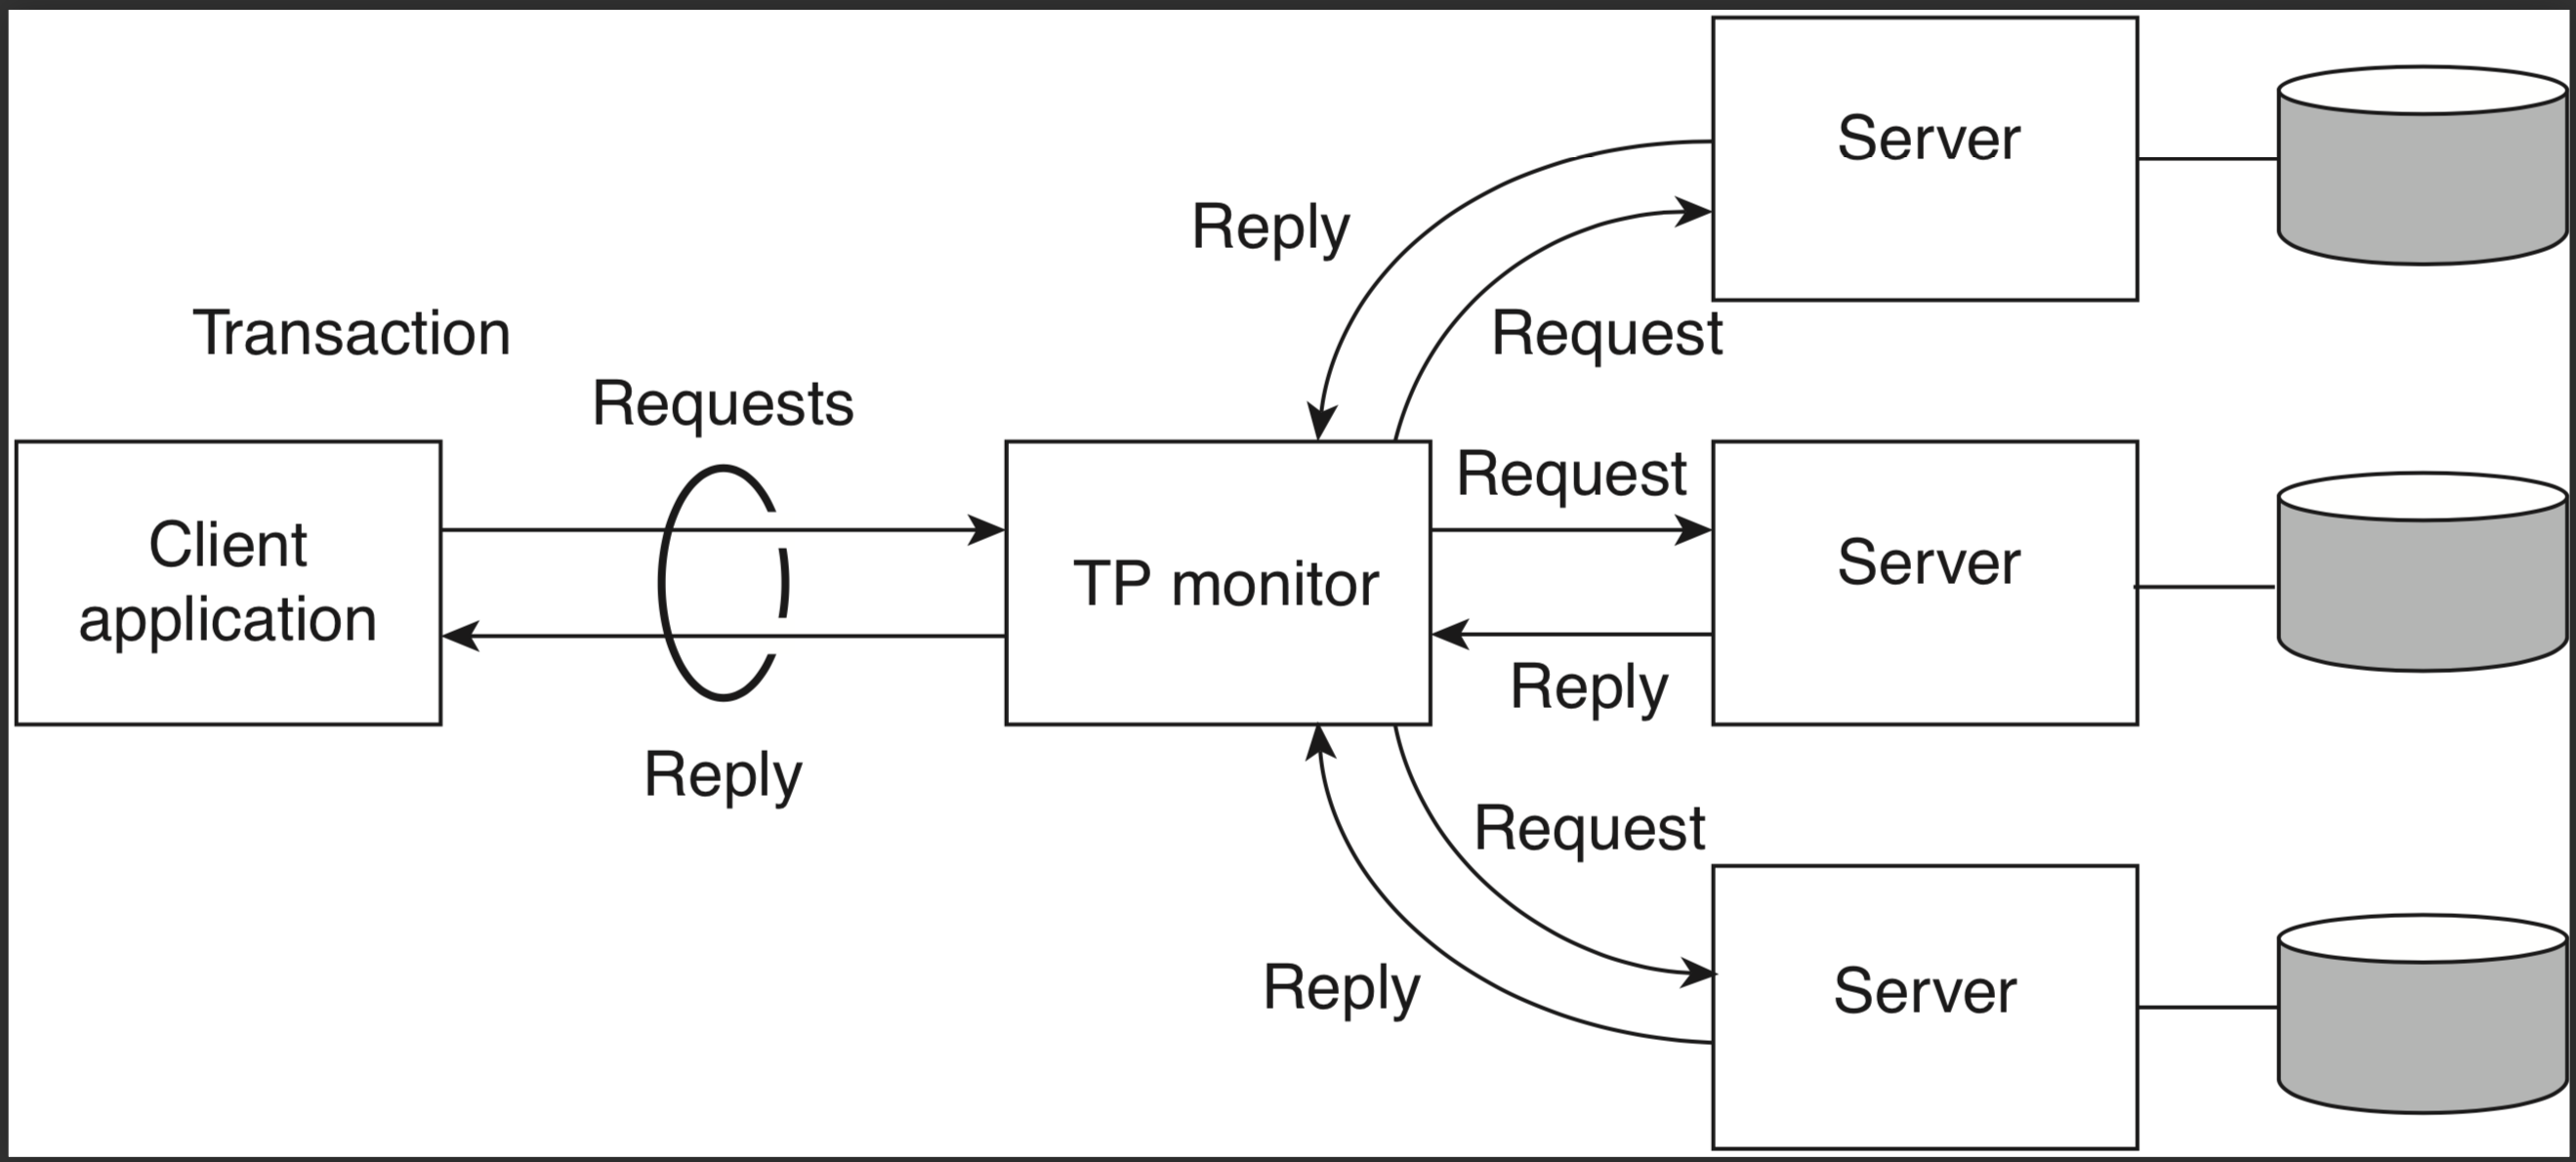
\includegraphics[width=.55\textwidth]{images/01-10}
\end{center}

\begin{itemize}
	\item beginTransaction(): tid (transaction id)
	\item operation(tid,op)	
	\item endTransaction(tid): Ok/NOk
	\item abortTransaction(tid)
\end{itemize}
\end{frame}


\begin{frame}{Transações Distribuídas}
Localmente, cada BD funciona como um sistema centralizado normal, usando abordagens otimistas ou pessimista para garantir consistência.

O grande problema no BD distribuído é garantir o \emph{acordo} na terminação.
\end{frame}

\subsection{Comprometimento Distribuído}

\begin{frame}{Atomicidade}
\begin{block}{O problema...}
	\begin{itemize}
		\item Transação $T$ acessa recursos nos Resource Managers (RM)
		\item Terminar com sucessos $T$ em todos os RM -- commit -- ou
		\item abortar $T$ em todos os RM
		\item ainda que enlaces de comunicação, nós e RM falhem, antes ou durante a terminação da transação.
	\end{itemize}
\end{block}

\alert{Comprometimento Distribuído}
\end{frame}

\begin{frame}{2PC}
\begin{itemize}
	\item Participante -- Resource Manager ``tocados'' pela transação
	\item Coordenador -- Transaction Manager
\end{itemize}
\end{frame}


\begin{frame}{Premissas}
\begin{itemize}
	\item Cliente decide quando iniciar o commit.
	\item Cada Participante faz commit ou abort da transação local.\\
		  Pode retornar Ok ou NOk.
	\item Coordenador não começa a commit até que a $T$ tenha terminado em todos os participantes e cliente tenha solicitado.
	\item Participantes falham por parada.
\end{itemize}
\end{frame}



\subsubsection{1 Phase Commit -- 1PC}
\begin{frame}[fragile]{Comprometimento em 1 Fase}
Aka 1-Phase Commit -- 1PC
\begin{itemize}
	\item Cliente envia \verb|endTransaction(tid)| para o Coordenador
	\item Coordenador envia mensagem para participantes ``comitarem'' \pause
	\item E se um participante retornar NOk? % enquanto outros retornam Ok?
	\item E se um participante não responder?
\end{itemize}
\end{frame}

\subsubsection{2-PC}

\begin{frame}[fragile]{Comprometimento em 2 Fases}
Aka 2-Phase Commit -- 2PC

\begin{itemize}
	\item Cliente envia \verb|endTransaction(tid)| para o coordenador
	\item coordenador envia mensagem para participantes se prepararem para terminar
	\item coordenador espera que todos se preparem ou digam se não podem
	\item coordenador envia \alert{ordem} de terminação
\end{itemize}
\end{frame}


\begin{frame}{Comprometimento}
\begin{itemize}
	\item Um Participante $P$ está pronto para commit se tiver todos os valores modificados por $T$ em memória estável e nenhuma razão para abortar a transação (outras transações conflituosas fizeram commit?)
	\item O Coordenador não pode começar a terminação até que todos os participantes estejam prontos.
	\item Se algum participante aborta, o Coordenador deve abortar. 
\end{itemize}

Problema de Acordo, mas não igual ao Consenso.
\end{frame}

\begin{frame}{2PC -- O Protocolo}
\begin{itemize}
	\item Fase 1
	\begin{itemize}
		\item A: Coordenador envia vote-request para participantes.
		\item B: Participante responde com vote-commit ou vote-abort para o coordenador; se vote-abort, aborta localmente.
	\end{itemize}
	\item Fase 2
	\begin{itemize}
		\item A: Coordenador coleta votos de todos os processos; se forem todos vote-commit, envia global-commit para os participantes e ok para o cliente
		\item B: Participantes esperam por global-commit ou global-abort
	\end{itemize}
\end{itemize}
\end{frame}


\begin{frame}{O Protocolo}
Coordenador \hfill Participante

\hfill
\includegraphics[width=.45\textwidth]{images/08-18a}
\hfill
\includegraphics[width=.45\textwidth]{images/08-18b}
\end{frame}

\begin{frame}{Falha no Participante}
Participante falha no estado $S$ e, ao se recuperar, identifica tal fato ao reprocessar o log de operações em memória durável.

Se está no estado
\begin{itemize}
	\item INIT: \pause nem sabia que a terminação começou. \pause Aborta unilateralmente, pois ou já abortaram ou vão abortar.\pause
	\item ABORT: havia votado abort ou recebido global-abort -- continua protocolo.
	\item COMMIT: estava pronto para terminar a transação com sucesso -- continua protocolo. 
	\item READY: \pause estava esperando por commit ou abort. \pause Precisa saber se coordenador enviou global-commit ou global-abort\pause -- consulta coordenador.
\end{itemize}
\end{frame}

\begin{frame}{2PC}
Por quê difícil?
\begin{itemize}
	\item E se $R_i$ falhar depois de ter se preparado?\pause
	\item E se $R_i$ falhar mas $R_j$ continuar funcionando?\pause
	\item E se todos estiverem desligados quando $R_i$ se recuperar?\pause
	\item E se $R_i$ estiver lento e parecer que a transação falhou?
\end{itemize}
\end{frame}


\begin{frame}{Falha no Participante}
\begin{itemize}
	\item READY: esperando por commit ou abort. Precisa saber se coordenador enviou global-commit our global-abort -- consulta coordenador.
\end{itemize}
	\alert{E se coordenador não estiver presente?} \pause 
	
Assumindo que participantes se conhecem \pause , contate participante $Q$	
	\begin{itemize}
		\item Se $Q$ em COMMIT\pause , vai para COMMIT
		\item Se $Q$ em ABORT\pause , vai para ABORT
		\item Se $Q$ em INIT\pause , ordena que Q aborte e, se confirmado, veja passo anterior
		\item Se $Q$ em READY\pause , consulta outro participante.
	\end{itemize}
\pause \alert{Se todos os participantes em READY?} \pause Possivelmente o coordenador já respondeu ao cliente.

\pause\alert{Precisa} esperar pelo coordenador.
\end{frame}

\begin{frame}{Falha no Coordenador}
O problema principal é: e se ninguém ouviu a decisão final do coordenador?

Neste caso, \pause o protocolo não pode continuar, enquanto o coordenador não retornar, pois se os RM abortarem, podem estar contradizendo algo dito ao cliente, por exemplo, "Sim, ATM, pode entregar o dinheiro", ou executando um comando que o cliente vê como anulado, como "Reenvie o pedido de mais 27 carros à fábrica."
\end{frame}

\begin{frame}{Recuperação do Coordenador}
	Ao se recuperar, o coordenador:
	\begin{itemize}
		\item sabe se começou a terminação de alguma transação
		\item sabe se já enviou alguma resposta final para as transações inacabadas
		\item sabe se já recebeu a confirmação de todos os participantes (se transação não estiver em aberto)
		\item reenvia a última mensagem das transações em aberto.
	\end{itemize}
\end{frame}

\begin{frame}{Otimizações}
	\begin{itemize}
		\item Participantes ``somente-leitura''
			\begin{itemize}
				\item Não se importa com a decisão; termina após fase 1.
				\item Responde com vote-commit-ro
			\end{itemize} 
		\item Abort presumido
			\begin{itemize}
				\item Se ocorrer timeout, coordenador envia global-abort a todos e esquece transação
				\item Se questionado, responde com global-abort.
			\end{itemize}
		\item Transferência de coordenação
			\begin{itemize}
				\item se houver somente um participante...
				\item vote-request-transfer
				\item participante responde com global-commit/global-abort
			\end{itemize} 
	\end{itemize}
\end{frame}

\begin{frame}{Coleta de Lixo}
Mesmo quando somente um participante falha...

Após receber decisão, o participante pode concluir e esquecer a transação. 

Mas e se o participante falho precisar se recuperar e todos os outros envolvidos tiverem esquecido a transação?

\pause Coleta de lixo só pode ser feita quando todos tiverem confirmado a execução da transação e, por isso, Fase 2b é necessária.
\end{frame}


\subsubsection{3-PC}

\begin{frame}{Comprometimento em Três Fases}
Estende o protocolo para permitir contornar  falha do coordenador.
\end{frame}


\begin{frame}{O Protocolo}
\begin{itemize}
	\item Fase 1a -- Coordenador envia vote-request para participantes.
	\item Fase 1b -- Participante responde com vote-commit ou vote-abort para o coordenador; se vote-abort, aborta localmente.
	\item Fase 2a -- Coordenador coleta votos de todos os processos; se forem todos vote-commit, envia \alert{prepare-commit} para os participantes; se não, global-abort e para.
	\item Fase 2b -- Participantes esperam por prepare-commit ou global-abort; se o primeiro, \alert{respondem com ready-commit}; se o segundo, param.
	\item Fase 3a -- coordenador espera por ready-commit de todos e então envia global-commit.
	\item Fase 3b -- participantes esperam por global-commit.
\end{itemize}
\end{frame}

\begin{frame}{O Protocolo}
Coordenador \hfill Participante

\includegraphics[width=.45\textwidth]{images/08-22a}
\hfill
\includegraphics[width=.45\textwidth]{images/08-22b}
\end{frame}


\begin{frame}{Falha no Participante}

$P$ consegue saber o que fazer após se recuperar da falha no estado READY ou PRE-COMMIT

\pause 
\begin{itemize}
	\item Participantes e coordenador não distam mais que um estado.
	\item Se alguém em READY, o coordenador não mandou global-commit ainda; Aborte.
	\item Se \alert{todos} em PRE-COMMIT, é possível comitar, comite.
	\item A execução dos passos anteriores tem que anular o poder do coordenador.
\end{itemize}
\pause \alert{Se todos os participantes em READY?}
\end{frame}

\begin{frame}{3PC x 2PC}
	\begin{itemize}
		\item 3PC -- Aumenta disponibilidade
		\item 2PC -- Falha do coordenador é ``corner case''
		\item 3PC -- Aumenta o custo do ``caminho feliz'' e por isso não é usado na prática
		\item Nenhum escala e não usá-los é uma das razões para o surgimento dos sistemas NoSQL
	\end{itemize}
\end{frame}

\subsubsection{Paxos-Commit}
\begin{frame}{Paxos-Commit}
Usa instâncias de Consenso Distribuído para votar. Se o consenso é tolerante a falhas e consistente, todos vêem o mesmo resultado na transação.
\end{frame}

\begin{frame}{O protocolo}
\begin{itemize}
	\item Para terminar a transação $T$, o coordenador envia request-commit a todos os participantes.
	\item Um participante $P$ propõe seu voto na instância $T_P$ de consenso.
	\item Todo participante $P$ espera pelas decisões das instâncias de consenso $T_i$ para todos os participantes $i$, inclusive si mesmo; se todas as decisões forem commit, o participante comita a transação.
	
	\item Se cansar de esperar por $T_Q$, o participante propõe abort em $T_Q$.
\end{itemize}
\end{frame}

\begin{frame}{Falha no Participante}
\begin{itemize}
	\item Se o participante falha antes de votar, então alguém votará abort por ele.
	\item Se o participante $P$ falha, ou é suspeito de, então é possível que dois votos diferentes tenham sido propostos em $T_P$;\pause isso não é um problema pois a decisão é a mesma para todos observando a instância.
	\item Após se recuperar, o participante recupera as decisões de todas as instâncias $T_i$ e termina apropriadamente.
\end{itemize}
\end{frame}

\subsection{Log Recuperável}
\begin{frame}{Log Recuperável}
Como garantir que o log poderá ser lido para recuperar o processo?
\end{frame}

\begin{frame}{Disco Duplicado}
\includegraphics[width=.7\textwidth]{images/08-23}

\begin{itemize}
	\item Dois discos iguais?
	\item Dados diferentes, mas ambos bons?
	\item Um bom outro estragado?
	\item Ambos estragados?
\end{itemize}
\end{frame}

